\documentclass[10pt,a4paper]{article}
\usepackage[utf8]{inputenc}
\usepackage{amsmath}
\usepackage{amsfonts}
\usepackage{amssymb}
\usepackage{a4wide} %Wider margins
\usepackage[english]{babel} %English dictionary for hyphenation and definitions, e.g. Table vs. Tabel
\usepackage[official]{eurosym} %Support for Euro-sign
\usepackage[utf8]{inputenc} %Support for internationalization, e.g. é vs.\’e
\usepackage{amsmath,amssymb,amsthm} %Support for mathematical formulas and symbols
\usepackage{fancyhdr} %Fancy headers
\usepackage{hyperref} %Creates clickable links
\usepackage{graphicx} %Support for grahpics
\usepackage{nopageno} %Support for removal of pagenumbers
\usepackage{tabularx}
\usepackage{enumitem}
\usepackage{xspace}
\usepackage{algorithm,algpseudocode}
\usepackage{float}
\usepackage{mathtools}
\usepackage[dvipsnames]{xcolor}
\usepackage[titletoc,toc,title]{appendix}
\usepackage{listings}
\usepackage{pdfpages}
\usepackage{attachfile2}
\graphicspath{ {./ThesisFigures/} }

\hypersetup{
    pdftitle={}, %PDF-file will be given a proper title when viewed in a reader
    hidelinks %PDF-file will be given clickable, yet not visible links when viewed in a reader
}
\newcommand{\documenttitle}{A Computational Biology Framework}
\newcommand{\documentsubtitle}{Creating a platform for biomedical engineers to efficiently do their research}


\newcommand{\true}{{\sc True}\xspace}
\begin{document}
	
	\begin{titlepage}
		
		\center
		
		\vspace*{3cm}
		
		\textbf{\huge \documenttitle}
		
		\textit{\LARGE \documentsubtitle}
		
		\vspace*{2cm}
		
		\large
		\centering
		T.P.A.~\textsc{Beishuizen}~(0791613)\\
		Biomedical Engineering - Computational Biology\\
		Data Engineering - Information Systems\\
		Eindhoven, University of Technology\\
		Email: \texttt{t.p.a.beishuizen@student.tue.nl}
		
		\vfill
		
		\vspace*{1cm}
		
		\today
		
	\end{titlepage}
	
	\tableofcontents
	
	%\newpage
	
	\pagestyle{fancy}
	%Abbreviations used by fancyhdr:
	%E Even page
	%O Odd page
	%L Left field
	%C Center field
	%R Right field
	%H Header
	%F Footer
	\fancyhead{} % clear all header fields
	\fancyfoot{} % clear all footer fields
	\renewcommand{\headrulewidth}{0.4pt}
	\renewcommand{\footrulewidth}{0.4pt}
	
	\fancyhead[L]{\rightmark}
	\fancyfoot[C]{\thepage}
	\fancyhead[R]{T.P.A. Beishuizen}
	
	
	\clearpage
	
	\section{Introduction}
	\label{sec:Introduction}
	
	% Quick explanation for graduation project
	At the Computational Biology department (cBio) of Biomedical Engineering (BME), many requests are made to analyse gathered data. This data usually stems from research in hospitals, but can also be from other BME groups and publicly available. Currently a standard is missing to efficiently analyse those data sets. With the vast number of data sets that are available, such a standard in the form of a framework on data analysis would be valuable. It would speed up projects and give them a higher chance to succeed the goal, due to improved efficiency. Before a framework can be made however a research must be done on all aspects that influence data analysis.
	
	% Layout graduation project
	First an extensive background on important topics for such a framework will be discussed. Four different parts are explained why they are important for the creation of such a framework. These parts are: biomedical data (data used for analysis), data analysis goal (how does a goal influence the choice of analysis), data analysis tools (which ones are usable) and at last biomedical knowledge (what engineers of BME and third parties already know about data analysis). After the extensive background research, a research question will be formulated with several sub-questions for each of the four parts and a hypothesis as an answer for each of the four questions.
	
	\section{Background}
	\label{sec:Background}
	
	% Biomedical engineering description.
	Biomedical engineering can be seen as a specific part of engineering with a wide variety of topics. These topics can be theoretical, non-experimental undertakings, but also state-of-the-art applications. Not only research and development can be used, but also implementation and operation. Combining all of these different parts in one definition is hard. \cite{bronzino2014biomedical} For this project, the focus is mainly on research and development, also known as knowledge discovery. \cite{bramer2007principles} 

	
	% Biomedical research summary
	When a biomedical engineer starts a project, at the start usually only a data set and the research goal are known. To achieve that certain goal from the data set, several different aspects influence the project's course and development. At first obviously the data itself is a big part of such an influencer as the research is restricted to limitations from it. Examples of such restrictions are multidimensionality, set size, data heterogeneity, missing feature values and population handling. The other obvious influencer is the main research goal. Since the biomedical engineer wants to achieve a certain goal, the approach outcome must match that goal for the research to be successful. Most goals are focused around either data mining, extracting relations from available data, or modelling, creating a model within data features. A third influencer is the availability of data analysis tools. The steps to take from data to goal do not only include an approach, but also a tool to execute it. The choice of a certain tool has a big impact on the project, as each one of them has its own advantages and disadvantages. The two most well known tools within BME are MATLAB and Python, however some engineers have used R, Java or C++ and there are still other possibilities. A last big influencer is the biomedical knowledge. What experience the scientist already has with similar projects can greatly influence the choice of approach and framework. Knowledge of the supervisor and publicly known information on the research subject from books and articles also influence the approach, as already known outcomes do not have to be researched again. 
	
	% Process steps for biomedical research
	Previous research projects on data mining have called for a model how to retrieve patterns from data collections. Frameworks to effectively do that have been proposed, usually with a number of steps.\cite{CIOS20021} These suggested frameworks do not specifically fit the cBio group though for being to broad \cite{fayyad1996knowledge} or being to specific. \cite{cios2000knowledge} A customized framework is needed. 
	
	\subsection{Biomedical Data}
	\label{subsec:BiomedicalData}
	
	% Introduction biomedical data
	A big aspect of choosing how to set up the data analysis is the data itself. The amount of data in the biomedical world is growing at an enormous rate, faster than biomedical engineers can analyse. Due to this rapid growth being uncontrollable, several additional challenges arose, aside being more than the biomedical world can handle. These challenges are mainly focused around data volume, dimensionality, complexity, heterogeneity and quality.\cite{chen2006medical, doi:10.1093/bib/bbx044}
	
	% Volume challenge
	Collecting data because it is possible can make data sets bigger than needed. Both in number of instances and features, data sets can be harder to understand or analyse when more is available.\cite{chen2006medical} This volume problem usually is tackled by taking sub-populations of the complete set. These sub-sets can either be focused around a part of the population (gender, age, race) or taken at random to still represent all of it. Due to the efficiency of analysis techniques and the rise in computational speed of servers\cite{blythe2008rise}, volume on its own becomes less of an issue. Volume does however become an issue when combining with heterogeneity and quality. \cite{Turkay2014, Holzinger2014} 
	
	% Dimensionality challenge
	Not all data sets have a high number of instances that cause a big data volume. Sometimes there are relatively few instances, while the number of features is proportionally high. \cite{dubitzky2007fundamentals} Usually many of those features are not relevant enough for the research, however are still used for testing. Trying to remove features that are not important, will greatly help finding relations between the others and create more knowledge about the research topic. Lowering the number of features also makes the data volume go down, so analysis should be easier. Mainly an optimal features set should be selected to obtain the best results. \cite{PENG201015}
	
	% Complexity challenge
	Biomedical data can also be very complex. Useful results may be present, however it can be very hard to obtain it. Examples of complex data are images, several biomedical signals and temporal data. Details of the useful results that are present in images can for example be very hard to detect, the temporal data can vary quite much over time and the biomedical signals can be hard to combine with static biomarkers. \cite{Yoo2012} This aspect can benefit from exchanging knowledge with other research areas that specialize in mining of those complex data sets. \cite{Turkay2014, bellazzi2011data}
	
	% Heterogeneity challenge
	The biggest challenge encompasses aligning different data sets. No standard for data sets is available and therefore data sets differ greatly from each other. Data is weakly structured or even unstructured \cite{Holzinger2014} and variables are processed differently due to other protocols or the collectors' preference of representation.\cite{Otasek2014} Also the variety of data is hard to combine when sources are fundamentally different. When parts of the data are images, another part is a table from the laboratory and a third part is textual remarks of the doctor, standardizing merging those three is much harder than merging three lab sets. Those merges are also very prone to errors, as imprecisions can be vastly different between those data sets. No tool can work directly with these raw data sets and preprocessing must almost definitely occur beforehand.\cite{CIOS20021, Turkay2014}
	
	% Quality challenge
	A last challenge is about data quality. The data is usually gathered by doctors and laboratory workers. Since the data is manually gathered by humans, the data have a relatively high error rate. Therefore the data can be quite noisy, values can be inconsistent, wrongly entered or even missing. \cite{CIOS20021} Not only human errors cause the data quality to drop, but the heterogeneity, as well. Two hospitals might have different protocols for the same treatment and sample different biomarkers for that protocol. Due to that difference, biomarkers may be missing for some of the entries. The time of data gathering is also a big factor as some biomarkers change greatly over time. The databases are usually also built for financial purposes and not for research, which can hurt the quality. \cite{Yoo2012}
	
	% Standardized database
	These challenges within the data are greatly discussed.\cite{bellazzi2011data} Many proposals to tackle them are made, however none is actually widely adopted, yet, as a global standard for databases. Also, with the uncontrolled growth in biomedical data, it will become hard to have such a standard recognised all over the world. \cite{Otasek2014, marenco2004qis, bichutskiy2006heterogeneous, sperzel1991biomedical, aubry1988design, Windridge2014}  
	
	\subsection{Data Mining}
	\label{subsec:DataMining}
	
	% Introduction data analysis goals
	Not only the data itself is important, but also the goal of a project. The data is analysed with a certain target in mind. This target off course heavily influences the data analysis approach that is taken. Two major aspects can be done for data analysis, data mining and modelling. For this project, the focus will be on data mining.
	
	% Data mining definition
	Data Mining has gained multiple definitions over the year. The most adopted definition is the following: “Data mining is the analysis of (often large) observational data sets to find unsuspected relationships and to summarize the data in novel ways that are both understandable and useful to the data owner." \cite{hand2001principles} As can be read in this definition, the main goal is find new and useful insights and patterns through datasets, that can be used in further decisions or hypotheses.\cite{chen2006medical, 7024124} It is one of the links that brings data and knowledge together.\cite{Yoo2012} A data mining project follows a certain layout. (Figure \ref{fig:ResearchSteps}), which in the end leads to further knowledge that aids the medical world.\cite{bramer2007principles} 
	
	\begin{figure}
		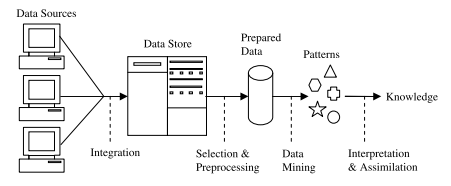
\includegraphics[scale=1.0]{ResearchSteps.png}
		\label{fig:ResearchSteps}
		\caption{A schematic overview how a project involving data mining is done. Multiple data sets are integrated in one database. Feature selection and preprocessing takes place to prepare the data. Then the data is mind to find patterns. These patterns are then interpreted and assimilated to discover knowledge on the subject.\cite{bramer2007principles}}
	\end{figure}
	
	% Types of data mining
	Since biomedical data is a wide scope, data mining has several specialisations in different direction. An example would be text data mining, used to find related articles with websites such as Pubmed and Google Scholar. These articles can mention similar genes, diseases or proteins and give additional information about them. Another examples would be microarray data mining. This type of data mining focuses on extracting entities and pathways that define a disease or other phenotype. Two other data mining types are proposed. One focuses on extracting useful information out of mass spectrometry data points, called proteomic data mining. A second focuses more on a molecular level and how these molecules would affect different cell types.\cite{YANG2012S16}
	
	% Reference to earlier made report
	Whichever splits are made in the data mining term for different areas in biomedical data analysis, the techniques are mostly based on statistical analysis and machine learning. A discussion of these two types has been made earlier (Appendix \ref{app:BiomedicalDataAnalysis}).
	
	\subsection{Data Mining Tools}
	\label{subsec:DataMiningTools}
	
	% Introduction data mining tools
	When applying several data mining algorithms to extract results from a data set, a certain tool has to be used that facilitates use of those algorithms. Several basic tools are available and widely used for this (Appendix \ref{app:BiomedicalDataAnalysis}). Since biomedical data has specific characteristics, separate tools or frameworks consisting of those tools are made. These are usually either made to create a database with a certain lay-out to put it in or to collect multiple algorithms and alter them specifically for biomedical cases. Many times both are connected as well, to optimize use.
	
	% Data set storage
	To store the data several projects are started. Famous project examples are the Human Genome Project (HGP) that tries to sequence the entire human genome\cite{sawicki1993human} or the Human Connectome Project (HCP) that focuses on the brain connectivity.\cite{van2012human} Both consist of an enormous amount of data that need to be stored and a tool is created for use in these project, for instance the ConnectomeDB for the HCP.\cite{marcus2011informatics}
	
	% Data set analysis
	
	
	
	The ability to share data effectively and efficiently is the starting point for successful
	analysis, and thus several attempts have been made to standardize formats for such
	data exchange: PSI-MI [35], BioPAX [42], KGML, SBML [40], GML, CML, and
	CellML [30]. \cite{Otasek2014}
	
	Resources for Studying Statistical Analysis
	of Biomedical Data and R \cite{Kobayashi2014}
	
	One aspect in comparing learning machines
	with each other deserves specific attention.
	If various machines are trained on
	training data, their performance can only
	be compared in a fair manner by applying
	all machines to the same test data. In this
	case, the above described procedures lead
	to valid estimates. \cite{bellazzi2011data}
	
	\subsection{Biomedical Knowledge}
	
	The traditional approach in biomedical science has been knowledge-driven and aimed at generating hypotheses from domain knowledge in a top-down fashion. Within biomedical data mining, one of the most
	interesting aspects is the exploitation of domain knowledge and the integration of different data sources in the data analysis process. As a matter of fact, data analysis is strongly empowered by the knowledge available in electronic format, which can be either already formalized, say through ontology and annotation repositories, or still informal but novel, as, for example, the one reported in Pubmed abstracts and papers\cite{bellazzi2011data}
	
	Perhaps the most distinctive feature that accompanies medical data analysis is knowledge; data analysis in medicine strives to discover new and useful knowledge, while using available knowledge to guide the process and incorporate it into discovered models. In these terms, we perform data analysis to extract new findings that either refine or supplement existing knowledge on the problem domain, a population of patients, or a specific patient under consideration. \cite{zupan2006knowledge}
	
	In data analysis, knowledge is represented either implicitly or explicitly. By explicit knowledge we refer to knowledge already established, formalized and coded within some knowledge base. Such knowledge is used in some way in the process of data analysis. Researchers in machine learning often refer to such knowledge as “background knowledge,” and use it in learning either in data preprocessing, feature selection or modeling. While this approach seems very promising in medical applications, the number of methods, tools and applications of such an approach are few. Most applications of data mining in medicine, for instance, have focused on building models directly from data and do not consider any explicitly represented knowledge in the process. These applications leave the interpretation of the models and the placement of any new information found in this way within the context of the available knowledge to analysts and domain experts. \cite{zupan2006knowledge}
	
	•The process of feature selection, or determining the set of variables that are thought best, a priori, to contribute to an analysis depends on an intimate familiarity with the problem domain. Numerous methods are available for reducing the feature space. Some are cognitive, such as expert panel verification, while others are computational. Results of either type of approach may be combined with existing knowledge to select most informative and interesting features that cover the problem from various angles.
	•The selection of preprocessing methods that may be required for certain data mining tasks depends on expertise in using not only the preprocessing methods but the data mining tools that may require the use of such methods. Discretization of continuous variables is an example of such a method. While the knowledge required for this task would appear to be primarily analytic, problem domain knowledge is needed as well, since some methods (such as discretization) can cause the loss of important scientific or clinical information.
	•The selection of an appropriate modeling methodology would also appear to be primarily in the analytic domain. However, the contribution of clinical or scientific knowledge to the modeling process cannot be underestimated. Examples of this are knowing when and how to model feature interactions. The selection and creation of these models requires collaboration between domain and analytic experts, due to the domain-specific realities of complex interactions and analysis-specific realities (and constraints) of computational complexity.
	•Finally, the selection of an appropriate methodology for presenting the results of an analysis requires expertise in such methodologies, but also in the clinical and scientific domain experts to whom the presentation is targeted. The primary goal of these methods is to reveal discovered knowledge in the optimal way to facilitate its communication to all members of the research team.\cite{zupan2006knowledge}
	
	\section{Research Question}
	
	\subsection{Hypotheses}
	
	\bibliography{../References/Citings} 
	\bibliographystyle{ieeetr}
	
	\appendix
	
	\clearpage
	
	\section{Biomedical Data Analysis}
	\label{app:BiomedicalDataAnalysis}
	
	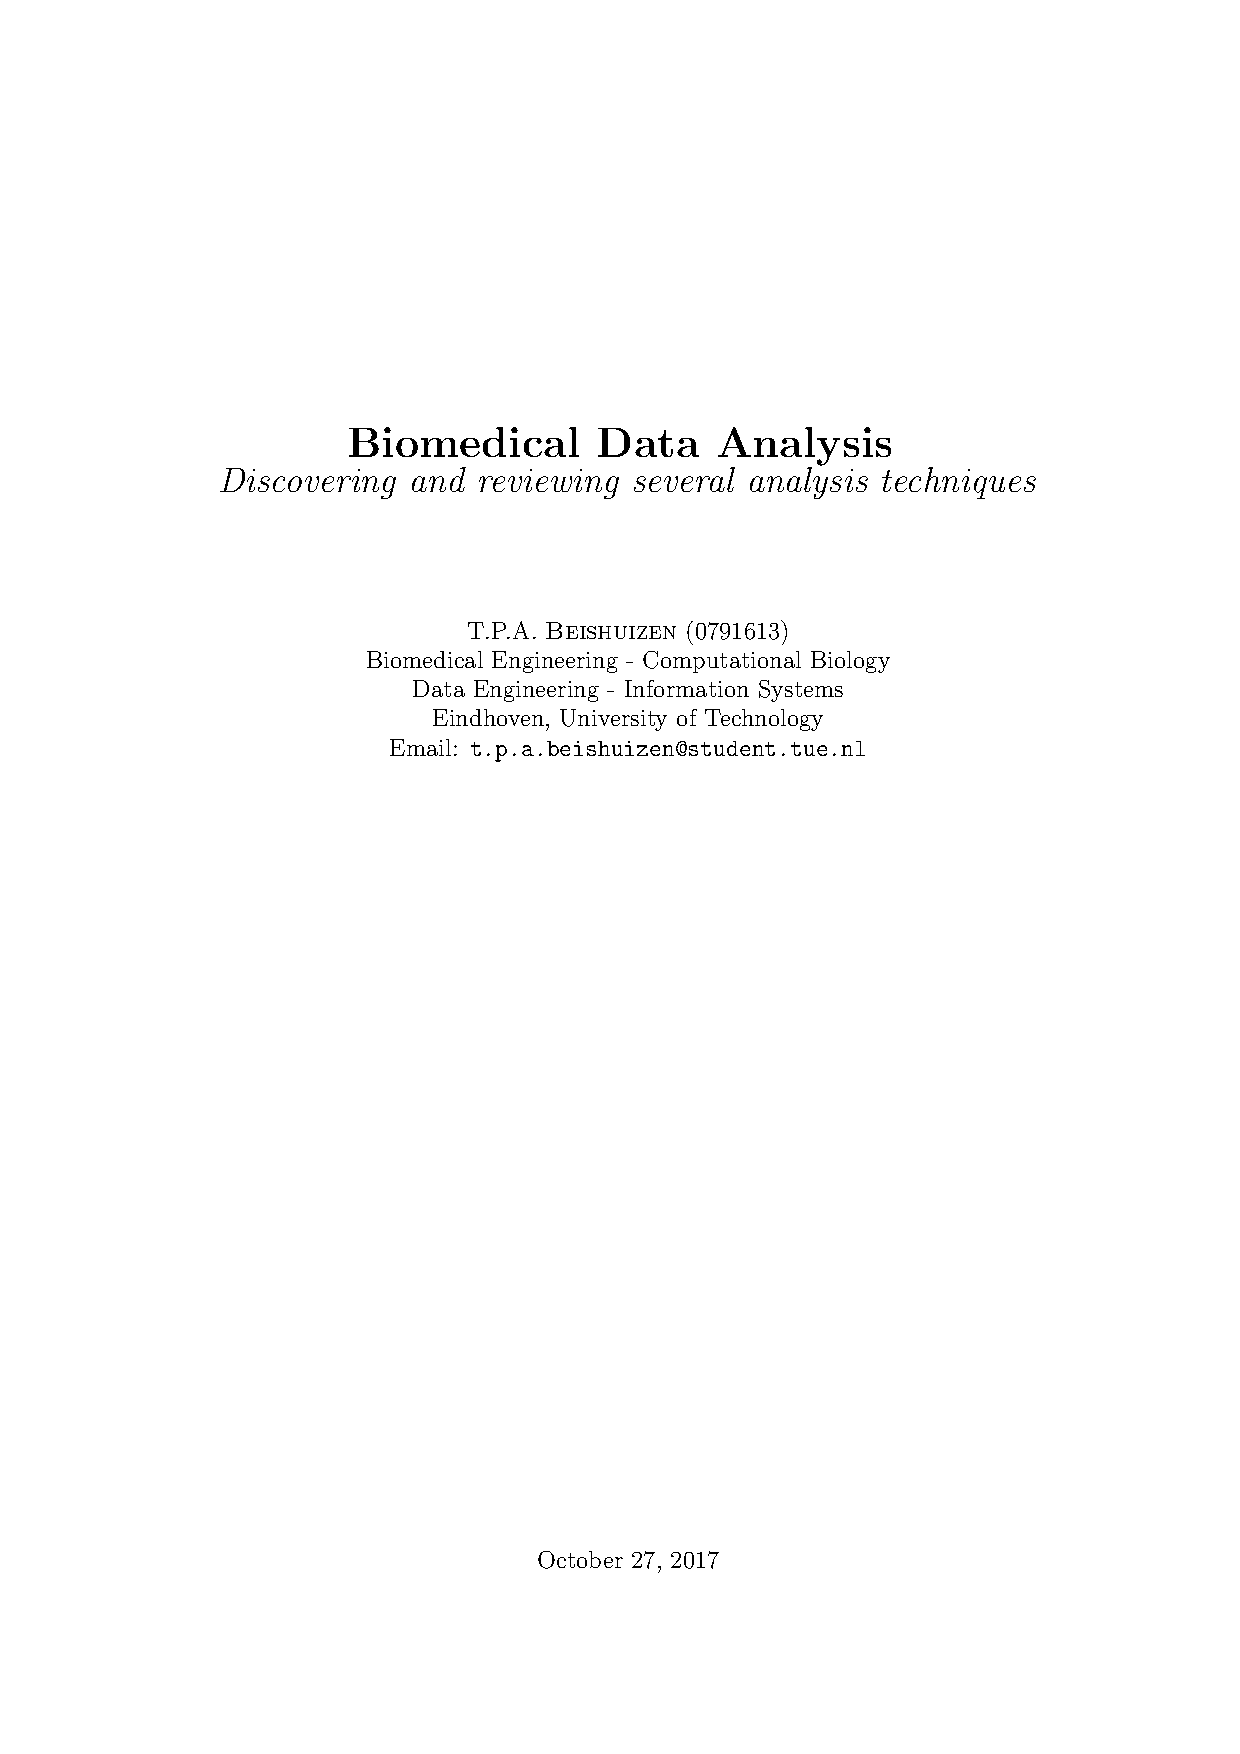
\includepdf[pages={1-22}]{../DataAnalysisThesis/BiomedicalDataAnalysis.pdf}
	
\end{document}
